\section{Уравение с разделёнными переменными}

$$ \frac{\di x}{g(x)} + \frac{\di y}{h(y)} = 0 $$
$$ U(x, y) = \ufint{g(x)} + \ufint[y]{h(y)} + C $$

\section{Уравнение с разделяющимися переменными}

$$ g_1(x)h_2(y)\di x + g_2(x)h_1(y)\di y = 0 $$
\antlersimp
\begin{multicols}{2}
    $$ \frac{g_1(x)}{g_2(x)}\di x + \frac{h_1(y)}{h_2(y)}\di y = 0 $$
    \columnbreak
    $$ \left[
    \begin{aligned}
        g_2(x) = 0 \quad \iff \quad x \equiv x_1, x_2, ... \\
        h_2(y) = 0 \quad \iff \quad y \equiv y_1, y_2, ...
    \end{aligned} \right. $$
    Это решения (т. к. $ \di x $ и $ g_2(x) $ одновременно обратятся в 0)
\end{multicols}

\section{Линейное уравнение}

$$ y' + p(x)y = \underset{\text{неоднородность}}{q(x)}, \qquad p(x), q(x) \in \Cont{\braket{a, b}} $$
\begin{itemize}
    \item Если $ q(x) \equiv 0 $, то уравнение $ y' + p(x)y = 0 $ называется линейным однородным (ЛОУ)
    \item Иначе $ y' + p(x)y = q(x) $ -- линейным неоднородным (ЛНУ)
\end{itemize}
$$ \underset{
    \begin{subarray}c
        \text{общее неоднородное} \\
        \text{(все реш. ЛНУ)}
    \end{subarray}}{y_{\text{ОН}}(x, C)} = \underset{
    \begin{subarray}c
        \text{общее однор.} \\
        \text{(все реш. ЛОУ)}
    \end{subarray}}{y_{\text{ОО}}(x, C)} + \underset{
    \begin{subarray}c
        \text{частное неоднор.} \\
        \text{(какое-то решение ЛНУ)}
    \end{subarray}}{y_{\text{ЧН}}(x, C)} $$
\begin{algo}
    \item Ищем $ y_{\text{ОО}} $:
    $$ y_{\text{ОО}} = Ce^{-\uint{p(x)}} $$
    \begin{note}
        Сюда, при допуске $ C = 0 $, входит $ y \equiv 0, \quad x \in \R $, ``потерянное'' при выводе этой формулы
    \end{note}
    \item Ищем $ y_{\text{ЧН}} $: \\
    Будем искать в виде
    $$ y_{\text{ЧН}} = C(x) \cdot e^{-\uint{p(x)}} $$
    \begin{remark}
        Эту формулу обязательно надо записать
    \end{remark}
    Подставим это в ЛНУ:
    $$ \underbrace{C'(x) \cdot e^{-\uint{p(x)}} + \cancel{C(x) \cdot e^{-\uint{p(x)}} \cdot \big( -p(x) \big)}}_{y_{\text{ЧН}}' \text{ как производная произведения}} + \cancel{p(x)\underbrace{C(x)e^{-\uint{p(x)}}}_{y_{\text{ЧН}}}} \equiv q(x) $$
    \begin{control}
        Второй и третий член \textbf{должны} сократиться
    \end{control}
    $$ C'(x) = e^{\uint{p(x)}}q(x) $$
    $$ C(x) = \uint{e^{\uint{p(x)}}q(x)} + \underset{(C_2)}0 $$
    Подставляем в формулу для $ y_{\text{ЧН}} $:
    $$ y_{\text{ЧН}} = \uint{e^{\uint{p(x)}}q(x)} \cdot e^{-\uint{p(x)}} $$
    \begin{remark}
        Если $ p(x) $ можно проинтегрировать (т. е. $ \uint{p(x)} = \xi(x) + C_1 $), нужно вместо $ C_1 $ записать какую-то конкретную константу (читайте: ноль). Мы ведь искали \textbf{частное} решение, а не континуум
    \end{remark}
    \item Ищем $ y_{\text{ОН}} $:
    $$ y_{\text{ОН}} = y_{\text{ОО}} + y_{\text{ЧН}} = Ce^{-\uint{p(x)}} + e^{-\uint{p(x)}} \cdot \uint{e^{\uint{p(x)}}q(x)} $$
    \begin{remark}
        Неберущийся неопределённый интеграл нужно записывать в виде интеграла с переменным верхним пределом, в нижнем пределе которого стоит выбранная числовая константа
    \end{remark}
    $$ y_{\text{ОН}} = e^{-P(x)} \bigg( C + \dint[s]{x_0}x{e^{P(s)}q(s)} \bigg), \qquad P(x) = \dint[t]{x_0}x{p(t)} $$
    \begin{remark}
        Не стоит здесь пользоваться готовой формулой. Нужно идти по алгоритму
    \end{remark}
\end{algo}

\section{Уравнение Бернулли}

$$ y' + p(x)y + r(x)y^\tau = 0, \qquad p(x), r(x) \in \Cont{\braket{a, b}} $$
\begin{remark}
    \hfill
    \begin{itemize}
        \item При $ \tau > 0 $ уравнение имеет тривиальное решение $ y \equiv 0, \quad x \in (a, b) $
        \item При $ \tau = 0, 1 $ -- это не уравнение Бернулли, а линейное
    \end{itemize}
\end{remark}
Стандартная замена:
$$ u = y^{1 - \tau}, \qquad u' = (1 - \tau)y^{-\tau}y' $$
\begin{remark}
    Здесь прямая замена не нужна -- просто делим на $ y^\tau $
\end{remark}
Получаем уравнение:
$$ (1 - \tau)^{-1}u' + p(x)u + r(x) = 0 $$

\section{Уравнение Риккати}

$$ y' + p(x)y + r(x)y^2 = q(x) $$
Иногда решается:
\begin{enumerate}
	\item Если известно какое-то частное решение: \\
    Пусть $ y = \eta(x) $ -- решение уравнения на некотором промежутке, то есть
    $$ \eta'(x) \equiv q(x) - p(x)\eta(x) - r(x)\eta^2(x), \qquad \text{ на } \braket{a, b} $$
    Замена $ y = z + \eta(x) $ преобразует наше уравнение в уравнение Бернулли
    $$ z' - \bigg( p(x) + 2r(x) \bigg)z + r(x)z^2 = 0 $$
    \item Если $ r(x) \ne 0 $ на $ \braket{a, b} $ и $ r(x) \in \Cont[1]{\braket{a, b}} $: \\
    Уравнение приводится к виду
    $$ u' + au^2 = s(x), \qquad a \ne 0 $$
    при помощи композиции двух замен:
    \begin{enumerate}
    	\item Линейная замена
        $$ y = \gamma(x) z, \qquad y' = \gamma'z + \gamma z', \qquad z = y\gamma^{-1} $$
        позволяет сделать коэффициент при квадратичном члене ненулевой константой
        \item Сдвигающая замена
        $$ z = u + \delta(x), \qquad z' = u' + \delta'x', \qquad u = z - \delta $$
        позволяет аннулировать линейный член, сохраняя коэффициент при $ z^2 $ неизменным
    \end{enumerate}
    \item Если уравнение имеет вид
    $$ u' = au^2 + cx^\sigma, \qquad \sigma \ne 0, -2 $$
    Оно называется специальным уравнением Риккати
    \begin{remark}
        При $ \sigma = 0 $ -- это уравнение с разделяющимися переменными, а при $ \sigma = -2 $ -- обобщённо-однородное \\
        В последнем случае замена
    $$ u = x^{-1}v^{-1} $$
    сводит уравнение к уравнению с разделяющимися переменными
    $$ xv' = -(cv^2 + v - a) $$
    \end{remark}
    Специальное уравнение Риккати интегрируется в квадратурах \bt{тогда и только тогда}, когда
    $$ k = \frac{\sigma}{2\sigma + 4} \in \Z \quad (k \ne 0 ), \qquad \text{то есть} \quad \sigma = \frac{4k}{1 - 2k} \quad (k \in \Z) $$
    \begin{algo}
    	\item Сделаем замену обеих переменных:
        $$
        \begin{cases}
        	x = t^{\faktor12 - k} \nimp[= t^\frac1{\sigma + 2}], \qquad t = x^{\frac2{1 - 2k}} > 0 \\
            u = z(t)t^{k - \faktor12} \nimp[= zt^{-\frac1{\sigma + 2}}], \qquad z = ux
        \end{cases} $$
        $$ \frac{\di u}{\di x} = \frac{\di (zt^{k - \half})}{\di t} \cdot \frac{\di t}{\di x} = \frac{t^{k - \half}\dot{z} + (k - \faktor12)t^{k - \faktor32}z}{(\faktor12 - k)t^{-\faktor12 - k}} = \frac{t^{2k}}{\faktor12 - k}\dot{z} - t^{2k - 1}z $$
        Получаем уравнение
        $$ t\dot{z} + \bigg( k - \half \bigg) z + a_0z^2 = c_0t, \qquad a_0 \define \bigg( \half - k \bigg) a, \quad c_0 \define \bigg( \half - k \bigg) c $$
        Это уравнение сводится к уравнению с разделяющимися переменными, если коэффициент при линейном члене равен $ -\faktor12 $
        \item ``Обнуляем'' $ k $: \\
        В зависимости от знака $ k $ используется одна из замен, сохраняющих структуру уравнения и позволяющих уменьшать $ |k| $ на 1:
        \begin{itemize}
        	\item $ k > 0 $:
            $$ z = a^{-1} + tv_1^{-1}, \qquad \dot{z} = v_1^{-1} - tv_1^{-2}\dot{v_1}, \qquad v_1 = t(x - a^{-1})^{-1} $$
            \item $ k < 0 $:
            $$ z = t(v_1 + d)^{-1}, \qquad \dot{z} = (v_1 + d)^{-1} - t(v_1 + d)^{-2}\dot{v_1}, \qquad v_1 = tz^{-1} - d $$
            $$ d \define \bigg( \half + k \bigg) \bigg( \half - k \bigg)^{-1}c^{-1} $$
        \end{itemize}
        В результате нескольких таких замен придём к уравнению
        $$ t\dot{v_k} + \bigg( -\half \bigg)v_k + a_kv_k^2 = c_kt $$
        \item Завершающая замена
        $$ v_k = t^{\faktor12}w, \qquad \dot{v_k} = \frac{t^{-\faktor12}w}2 - t^{\faktor12}\dot{w}, \qquad w = t^{-\faktor12}v_k $$
        приводит уравнение к уравнению с разделяющимися переменными
        $$ t^{\faktor12}\dot{w} = a_kw^2 - c_k $$
    \end{algo}
\end{enumerate}

\section{Однородное уравнение}

\begin{definition}
    $ h(x, y) $ называется однородной функцией степени $ k $, если $ h(sx, sy) = s^kh(x, y) $
\end{definition}
Уравнения
$$ y' = h \bigg( \frac{y}x \bigg) \qquad \text{и} \qquad M(x, y)\di x + N(x, y)\di y, \qquad M, N \text{ -- однородные порядка } k $$
называются однородными (порядка 0) \\
То есть, уравнение однородное, если каждое его слагаемое имеет одну и ту же суммарную степень по $ x $ и $ y $ \\
Стандартная замена:
$$ y(x) = u(x)x, \qquad
\begin{vars}
    y' = u'x + u \\
    \di y = u\di x + x\di u
\end{vars}, \qquad u = x^{-1}y $$
\begin{control}
    После замены \textbf{каждое} слагаемое должно содержать $ x^k $
\end{control}
Сокращаем на $ x^k $, группируем слагаемые при $ \di x $ и $ \di y $ -- получаем уравнение с разделяющимися переменными

\section{Дробно-линейное уравнение}

$$ y' = \bigg( \frac{a_1x + b_1y + c_1}{a_2x + b_2y + c_2} \bigg) $$
Числитель и значенатель задают прямые, пусть $ l_1 = a_1x + b_1y + c_1, \quad l_2 = a_2x + b_2y + c_2 $ \\
Возможны два случая:
\begin{itemize}
    \item $
    \begin{vmatrix}
        a_1 & b_1 \\
        a_2 & b_2
    \end{vmatrix} \ne 0 $
    \begin{figure}[!ht]
        \begin{tikzpicture}
            \draw[name path=l1] (-1, -1) -- (1, 1) node[right]{$ l_1 $};
            \draw[name path=l2] (-1, 1) -- (1, -1) node[right]{$ l_2 $};
            \node[name intersections={of=l1 and l2}] at (intersection-1)[left]{$ (x_*, y_*) $};
        \end{tikzpicture}
    \end{figure} \\
    Пусть $ (x_*, y_*) $ -- решение системы
    $$
    \begin{cases}
        a_1x + b_1y + c_1 = 0 \\
        a_2x + b_2y + c_2 = 0
    \end{cases} $$
    или, что то е самое, точка пересечения прямых $ l_1 $ и $ l_2 $ \\
    После сдвига начала координат в точку $ (x_*, y_*) $ прямые не будут иметь свободных членов \\
    Итак, после замены
    $$ u = x - x_*, \qquad v = y - y_*, \qquad \di u = \di x, \qquad \di v = \di y $$
    или $ y'(x) = v'(u) $ получаем однородное уравнение
    $$ v' = h \bigg( \frac{a_1u + b_1v}{a_2u + b_2v} \bigg) $$
    \item $
    \begin{vmatrix}
        a_1 & b_1 \\
        a_2 & b_2
    \end{vmatrix} = 0 $
    \begin{figure}[!ht]
        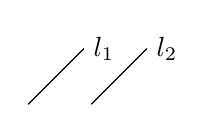
\begin{tikzpicture}
            \draw (0, 0) -- +(45:1) node[right]{$ l_1 $};
            \draw (0.8, 0) -- +(45:1) node[right]{$ l_2 $};
        \end{tikzpicture}
    \end{figure} \\
    Тогда $ b_1 \ne 0 $ и $ \dfrac{b_2}{b_1} = \dfrac{a_2}{a_1} = k $ \\
    В этом случае замена
    $$ u = a_1x + b_1y, \qquad y = \frac1{b_1}(u - a_1x), \qquad y' = \frac1{b_1}(u' - a_1) $$
    сразу приводит уравнение к уравнению с разделяющимися переменными:
    $$ u' = b_1h \bigg( \frac{u + c_1}{ku + c_2} \bigg) + a_1 $$
\end{itemize}

\section{Обощённо-однородное уравнение}

\begin{definition}
    Уравнение называется обощённо-однородным, если каждое его слагаемое имеет один и тот же суммарный порядок по $ x $ и $ y $ при условии, что $ x, \di x $ имеют порядок 1, а $ y, \di y $ -- порядок $ m \ne 0 $
\end{definition}
Тогда $ y' = \frac{\di x}{\di y} $ имеет порядок $ m - 1 $ \\
Аргументы входящих в уравнение функций типа логарифма или тригонометрических должны иметь нулевой порядок \\
Таким образом, чтобы установить, является ли уравнение обобщённо-однородным, надо приравнять порядки всех слагаемых, получая систему многих уравнений с одной неизвестной $ m $. Если повезёт, такое число $ m $ найдётся. Тогда замена
$$ y = z^m, \qquad y' = mz^{m - 1}z', \qquad z = y^{\faktor1m} $$
сведёт уравнение к однородному, но не всегда:

\begin{undefthm}{Проблема}
    Проблема возникает, когда $ y $ может принимать значения разных знаков (ОДЗ этого не запрещает), и отсутсвует инвариантность относительно замены $ y = -\vawe{y} $
\end{undefthm}

В таком случае надо отдельно проверить $ y(x) \equiv 0 $ \\
Дальше возможно три случая:
\begin{itemize}
	\item Общий: \\
    Замена
    $$ y = (xu)^m, \qquad y' = m(xu)^{m - 1}(u + xu'), \qquad u = x^{-1}y^{\faktor1m} $$
    приведёт к уравнению с разделяющимися переменными (но придётся решить два раза для разных знаков $ y $)
    \item Если $ \exist q \in \Z : m = 2q $ \\
    Делаем замену
    $$ y = x^{2q}u, \qquad y' = 2qx^{2q - 1}u + x^{2q}u', \qquad u = x^{-2q}y $$
    Она не фиксирует знак $ y $, так что не придётся решать уравнение второй раз \\
    Также получаем сразу уравнение с разделяющимися переменными
    \item Если $ \exist q \in \Z : m = (2q)^{-1} $, при этом $ x $ тоже меняет знак, и отсутсвует инвариантность относительно замены $ x = -\vawe{x} $ \\
    Надо следать замену
    $$ y = |x|^{\frac1{2q}}u, \qquad y' = \sigma \frac{\di y}{\di |x|} = \sigma \bigg( (2q)^{-1}|x|^{\frac1{2q} - 1}u + |x|^{\frac1{2q}}u' \bigg), \quad \text{где } u' = \frac{\di u}{\di |x|}, \qquad u = |x|^{-\frac1{2q}}y $$
    где $ \sigma = \operatorname{sign} x $ \\
    Получается уравнение с разделяющимися переменными и параметром $ \sigma $
    \begin{control}
    	В ответе не должно остаться $ \sigma $ (т. е. каждая $ \sigma $ должна ``найти'' свой $ |x| $)
        \begin{note}
        	$ \sigma |x| = x $
        \end{note}
    \end{control}
\end{itemize}
